\documentclass[10pt, aspectratio=169]{beamer}
\usefonttheme{professionalfonts}

\mode<presentation>
{
  \usetheme{Berkeley}
  \usecolortheme{beaver}
  \usefonttheme{default}
  \setbeamertemplate{navigation symbols}{}
  \setbeamertemplate{caption}[numbered]
} 

\setbeamertemplate{footline}{%
  \leavevmode%
  \hbox{%
    \begin{beamercolorbox}[wd=.85\paperwidth,ht=2.5ex,dp=1ex,left]{author in head/foot}%
      \usebeamerfont{author in head/foot}Maxx Seminario, Electronic Circuits, Spring 2026%
    \end{beamercolorbox}%
    \begin{beamercolorbox}[wd=.15\paperwidth,ht=2.5ex,dp=1ex,right]{date in head/foot}%
      \hspace*{0.5em}\insertframenumber{} / \inserttotalframenumber\hspace*{0.5em}%
    \end{beamercolorbox}%
  }%
  \vskip0pt%
}

\usepackage[english]{babel}
\usepackage[utf8x]{inputenc}
\usepackage{tikz}
\usetikzlibrary{shapes.geometric}
\usepackage{pgfplots}
\usepackage{array}
\usepackage{makecell}
\usepackage{verbatim}
\usepackage{graphicx}
\usepackage{subcaption}
\usepackage{amsfonts}
\usepackage{amsmath}
\usepackage{bm}
\usepackage{epstopdf}
\usepackage{circuitikz}
\usepackage{caption}
\usepackage{multirow}
\captionsetup{compatibility=false}
\usepackage[absolute,overlay]{textpos}
\usetikzlibrary{calc}
\usetikzlibrary{pgfplots.fillbetween, backgrounds}
\usetikzlibrary{positioning}
\usetikzlibrary{pgfplots.groupplots}
\usetikzlibrary{plotmarks}
\usetikzlibrary{calc}
\usetikzlibrary{patterns}
\usepgfplotslibrary{groupplots}
\pgfplotsset{compat=newest} 

\usepackage{hyperref}
\definecolor{BeaverRed}{RGB}{179,38,38} 
\hypersetup{
    colorlinks=true,
    linkcolor=BeaverRed,
    filecolor=magenta,      
    urlcolor=cyan,
}

% Added by Maxx Seminario - for colored icons in itemize labels
\usepackage{wasysym} 
\newcommand{\neutralface}{%
  \tikz[baseline=-0.6ex]{
    \draw (0,0) circle (0.9ex);
    \fill (-0.35ex,0.25ex) circle (0.12ex);
    \fill ( 0.35ex,0.25ex) circle (0.12ex);
    \draw (-0.35ex,-0.25ex) -- (0.35ex,-0.25ex);
  }%
}

\newcommand{\baditem}{\textcolor{red! 70! black}{\frownie}}
\newcommand{\gooditem}{\textcolor{green!60!black}{\smiley}}
\newcommand{\mehitem}{\textcolor{orange!80!black}{\neutralface}}

% =========================
% Solution toggle 
% =========================
\newif\ifshowsolutions
\showsolutionstrue   %  compile WITH solutions
%\showsolutionsfalse %  compile WITHOUT solutions

% =========================
% Document Information
% =========================
\title[PN Junction Under Bias]{PN Junction External Under Bias}
\subtitle{Forward Bias, Reverse Bias, and Breakdown}
\author{Maxx Seminario}
\institute{University of Nebraska-Lincoln}
\date{Spring 2026}

\begin{document}

\begin{frame}
  \titlepage
\end{frame}

\section{Introduction}

\begin{frame}{Lecture Overview}
    
    \begin{columns}[t]
    \column{0.48\textwidth}
        \textbf{Previously}: PN Junction at Equilibrium
        
        \begin{itemize}
            \item Built-in potential $V_{bi}$
            \item Depletion region formation
            \item Flat Fermi level
            \item Zero net current
        \end{itemize}
        
        \vspace{0.5cm}
        
        \textbf{Today}: PN Junction Under Bias
        
        \begin{itemize}
            \item Apply external voltage
            \item Break equilibrium
            \item Control current flow
            \item Understand diode operation
        \end{itemize}
        
    \column{0.48\textwidth}
        \begin{block}{Lecture Objectives}
            \begin{itemize}
                \item Review equilibrium condition
                \item Analyze forward bias operation
                \item Analyze reverse bias operation
                \item Understand breakdown mechanisms
                \item Derive diode I-V characteristics
            \end{itemize}
        \end{block}
        
        \vspace{0.3cm}
        
        \textbf{Applications}:
        \begin{itemize}
            \item Rectifier circuits
            \item Voltage regulation (Zener diodes)
            \item Switching circuits
            \item Power supplies
        \end{itemize}
        
    \end{columns}
    
\end{frame}

\section{Review: Equilibrium}

\begin{frame}{Review: Energy Band Diagram at Thermal Equilibrium}
    
    \begin{center}
    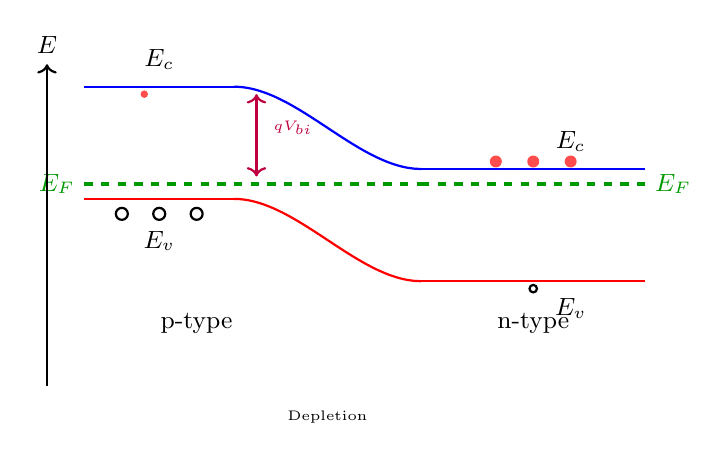
\begin{tikzpicture}[scale=0.95]
        % p-type region (x: 0 to 2, Ec at 3, Ev at 1.5)
        \begin{scope}[xshift=0cm]
            % Conduction band - flat in p-region
            \draw[thick, blue] (0,3) -- (2,3);
            \node[above, font=\small] at (1,3.1) {$E_c$};
            
            % Valence band - flat in p-region
            \draw[thick, red] (0,1.5) -- (2,1.5);
            \node[below, font=\small] at (1,1.2) {$E_v$};
            
            % Fermi level (flat at equilibrium)
            \draw[very thick, green!60!black, dashed] (0,1.7) -- (2,1.7);
            \node[left, font=\small, green!60!black] at (0,1.7) {$E_F$};
            
            % Holes in p-region
            \foreach \x in {0.5,1.0,1.5} {
                \draw[fill=white, thick] (\x,1.3) circle (0.08cm);
            }
            
            % Few electrons in p-region
            \fill[red!70] (0.8,2.9) circle (0.05cm);
            
            \node[below, font=\small] at (1.5,0.1) {p-type};
        \end{scope}
        
        \begin{scope}[xshift=0cm]
            % Conduction band sigmoid
            \draw[thick, blue, domain=2:4.5, samples=30, smooth] 
                plot (\x, {3 - 1.1*(3*(((\x-2)/2.5)^2) - 2*(((\x-2)/2.5)^3))});
            
            % Valence band sigmoid
            \draw[thick, red, domain=2:4.5, samples=30, smooth] 
                plot (\x, {1.5 - 1.1*(3*(((\x-2)/2.5)^2) - 2*(((\x-2)/2.5)^3))});
            
            % Fermi level continues flat
            \draw[very thick, green!60!black, dashed] (2,1.7) -- (4.5,1.7);
            
            \node[below, font=\tiny] at (3.25,-1.2) {Depletion};
            
            % Draw potential barrier
            \draw[<->, thick, purple] (2.3,1.8) -- (2.3,2.9);
            \node[right, font=\tiny, purple] at (2.4,2.45) {$qV_{bi}$};
        \end{scope}
        
        % n-type region (x: 4.5 to 7.5, Ec at 1.9, Ev at 0.4)
        \begin{scope}[xshift=0cm]
            % Conduction band - flat in n-region
            \draw[thick, blue] (4.5,1.9) -- (7.5,1.9);
            \node[above, font=\small] at (6.5,2.0) {$E_c$};
            
            % Valence band - flat in n-region
            \draw[thick, red] (4.5,0.4) -- (7.5,0.4);
            \node[below, font=\small] at (6.5,0.3) {$E_v$};
            
            % Fermi level
            \draw[very thick, green!60!black, dashed] (4.5,1.7) -- (7.5,1.7);
            \node[right, font=\small, green!60!black] at (7.5,1.7) {$E_F$};
            
            % Electrons in n-region
            \foreach \x in {5.5,6.0,6.5} {
                \fill[red!70] (\x,2.0) circle (0.08cm);
            }
            
            % Few holes in n-region
            \draw[fill=white, thick] (6.0,0.3) circle (0.05cm);
            
            \node[below, font=\small] at (6.0,0.1) {n-type};
        \end{scope}
        
        % Energy axis
        \draw[->, thick] (-0.5,-1) -- (-0.5,3.3) node[above, font=\small] {$E$};
        
    \end{tikzpicture}
    \end{center}
    
    \begin{itemize}
        \item \textbf{No applied voltage}: $V_A = $ open circuit
        \item \textbf{Flat Fermi level}: System in thermal equilibrium
        \item \textbf{Barrier height}: $qV_{bi}$ prevents carrier diffusion
    \end{itemize}
    
\end{frame}

\begin{frame}{Review: Drift and Diffusion at Equilibrium}
    
    \begin{center}
    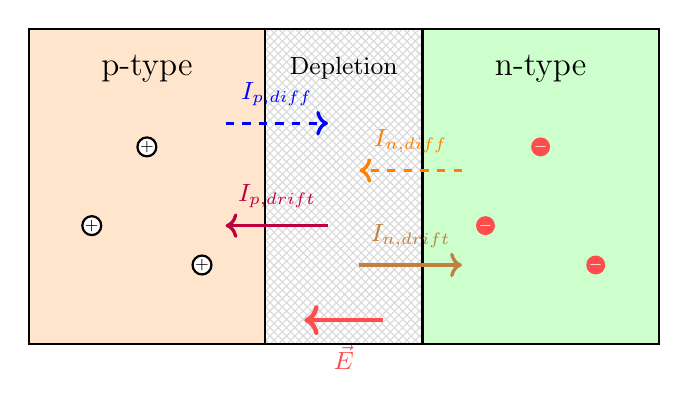
\begin{tikzpicture}[scale=1.0]
        % p-type region
        \draw[thick, fill=orange!20] (0,0) rectangle (3,4);
        \node[font=\large] at (1.5,3.5) {p-type};
        
        % Depletion region
        \draw[thick, fill=yellow!30, pattern=crosshatch, pattern color=gray!30] (3,0) rectangle (5,4);
        \node[font=\small] at (4,3.5) {Depletion};
        
        % n-type region
        \draw[thick, fill=green!20] (5,0) rectangle (8,4);
        \node[font=\large] at (6.5,3.5) {n-type};
        
        % Holes in p-region
        \foreach \x/\y in {0.8/1.5, 1.5/2.5, 2.2/1.0} {
            \draw[fill=white, thick] (\x,\y) circle (0.12cm) node[black, font=\tiny] {$+$};
        }
        
        % Electrons in n-region
        \foreach \x/\y in {5.8/1.5, 6.5/2.5, 7.2/1.0} {
            \fill[red!70] (\x,\y) circle (0.12cm);
            \node[white, font=\tiny] at (\x,\y) {$-$};
        }
        
        % Diffusion currents
        \draw[->, very thick, blue, dashed] (2.5,2.8) -- (3.8,2.8);
        \node[above, font=\small, blue] at (3.15,2.9) {$I_{p,diff}$};
        
        \draw[->, very thick, orange, dashed] (5.5,2.2) -- (4.2,2.2);
        \node[above, font=\small, orange] at (4.85,2.3) {$I_{n,diff}$};
        
        % Drift currents
        \draw[->, very thick, purple] (3.8,1.5) -- (2.5,1.5);
        \node[above, font=\small, purple] at (3.15,1.6) {$I_{p,drift}$};
        
        \draw[->, very thick, brown] (4.2,1.0) -- (5.5,1.0);
        \node[above, font=\small, brown] at (4.85,1.1) {$I_{n,drift}$};
        
        % Electric field arrow
        \draw[->, ultra thick, red!70] (4.5,0.3) -- (3.5,0.3);
        \node[below, font=\small, red!70] at (4,0.1) {$\vec{E}$};
        
    \end{tikzpicture}
    \end{center}
    
    \vspace{-0.1cm}
    
    \begin{block}{At Equilibrium ($V_A = $ open circuit)}
        \begin{itemize}
            \item $I_{p,diff} = -I_{p,drift}$ (currents cancel)
            \item $I_{n,diff} = -I_{n,drift}$ (currents cancel)
            \item $I_{total} = 0$ (no net current)
        \end{itemize}
    \end{block}
    
\end{frame}

\section{Forward Bias}

\begin{frame}{Forward Bias: Circuit Configuration}
    
    \begin{columns}[t]
    \column{0.48\textwidth}
        \textbf{Definition}:
        \begin{itemize}
            \item Connect positive terminal to p-side
            \item Connect negative terminal to n-side
            \item Applied voltage: $V_A > 0$
        \end{itemize}
        
        \vspace{0.3cm}
        
        \textbf{Effect on Junction}:
        \begin{itemize}
            \item Reduces barrier height
            \item Barrier becomes: $q(V_{bi} - V_A)$
            \item Increases carrier injection
            \item Large current flows
        \end{itemize}
        
    \column{0.48\textwidth}
        \begin{center}
        \begin{circuitikz}[scale=0.8]
            % Battery
            \draw (0,0) to[battery1, l=$V_A > 0$, invert] (0,2);
            
            % PN junction diode
            \draw (0,2) -- (1,2);
            \draw (1,0.5) rectangle (2,3.5);
            \fill[orange!20] (1,0.5) rectangle (1.5,3.5);
            \fill[green!20] (1.5,0.5) rectangle (2,3.5);
            \node at (1.25,2) {p};
            \node at (1.75,2) {n};
            \draw (2,2) -- (3,2);
            
            % Complete circuit
            \draw (3,2) -- (3,0) -- (0,0);
            
            % Labels
            \node[above] at (0.5,2.1) {$+$};
            \node[above] at (2.5,2.1) {$-$};
            
            % Current arrow
            \draw[->, very thick, red] (1,3.8) -- (2,3.8);
            \node[right, font=\small] at (1,4.2) {$I > 0$};
            
        \end{circuitikz}
        \end{center}
        
        % \vspace{0.3cm}
        
        \begin{block}{Key Point}
            Forward bias \textbf{reduces} the potential barrier, allowing majority carriers to flow across junction.
        \end{block}
        
    \end{columns}
    
\end{frame}

\begin{frame}{Forward Bias: Energy Band Diagram}
    
    \begin{center}
    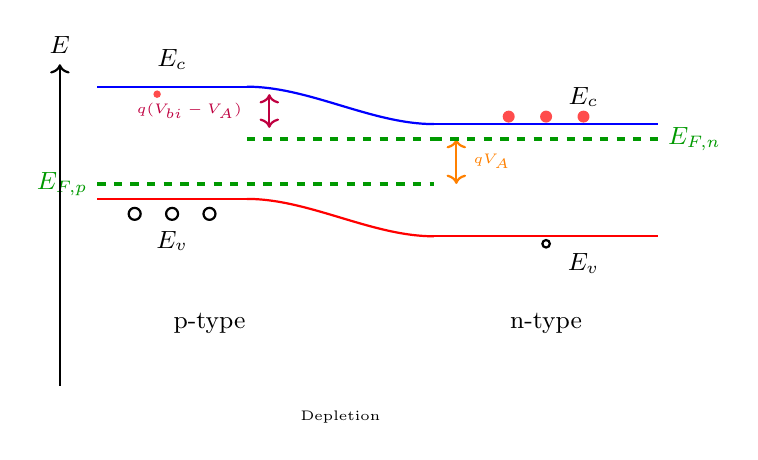
\begin{tikzpicture}[scale=0.95]
        % p-type region
        \begin{scope}[xshift=0cm]
            \draw[thick, blue] (0,3) -- (2,3);
            \node[above, font=\small] at (1,3.1) {$E_c$};
            
            \draw[thick, red] (0,1.5) -- (2,1.5);
            \node[below, font=\small] at (1,1.2) {$E_v$};
            
            % Fermi level - NOT flat under bias
            \draw[very thick, green!60!black, dashed] (0,1.7) -- (2,1.7);
            \node[left, font=\small, green!60!black] at (0,1.7) {$E_{F,p}$};
            
            % More holes
            \foreach \x in {0.5,1.0,1.5} {
                \draw[fill=white, thick] (\x,1.3) circle (0.08cm);
            }
            
            \fill[red!70] (0.8,2.9) circle (0.05cm);
            
            \node[below, font=\small] at (1.5,0.1) {p-type};
        \end{scope}
        
        % Depletion region - REDUCED barrier
        \begin{scope}[xshift=0cm]
            % Reduced band bending (only 0.5 eV instead of 1.1 eV)
            \draw[thick, blue, domain=2:4.5, samples=30, smooth] 
                plot (\x, {3 - 0.5*(3*(((\x-2)/2.5)^2) - 2*(((\x-2)/2.5)^3))});
            
            \draw[thick, red, domain=2:4.5, samples=30, smooth] 
                plot (\x, {1.5 - 0.5*(3*(((\x-2)/2.5)^2) - 2*(((\x-2)/2.5)^3))});
            
            % Fermi levels split (p-side lower, n-side higher for forward bias)
            \draw[very thick, green!60!black, dashed] (2,1.7) -- (4.5,1.7);
            \draw[very thick, green!60!black, dashed] (2,2.3) -- (4.5,2.3);
            
            \node[below, font=\tiny] at (3.25,-1.2) {Depletion};
            
            % Reduced barrier
            \draw[<->, thick, purple] (2.3,2.45) -- (2.3,2.9);
            \node[right, font=\tiny, purple] at (0.4,2.68) {$q(V_{bi}-V_A)$};
            
            % Applied voltage arrow (between the two Fermi levels)
            \draw[<->, thick, orange] (4.8,1.7) -- (4.8,2.3);
            \node[right, font=\tiny, orange] at (4.9,2.0) {$qV_A$};
        \end{scope}
        
        % n-type region
        \begin{scope}[xshift=0cm]
            \draw[thick, blue] (4.5,2.5) -- (7.5,2.5);
            \node[above, font=\small] at (6.5,2.6) {$E_c$};
            
            \draw[thick, red] (4.5,1.0) -- (7.5,1.0);
            \node[below, font=\small] at (6.5,0.9) {$E_v$};
            
            \draw[very thick, green!60!black, dashed] (4.5,2.3) -- (7.5,2.3);
            \node[right, font=\small, green!60!black] at (7.5,2.3) {$E_{F,n}$};
            
            \foreach \x in {5.5,6.0,6.5} {
                \fill[red!70] (\x,2.6) circle (0.08cm);
            }
            
            \draw[fill=white, thick] (6.0,0.9) circle (0.05cm);
            
            \node[below, font=\small] at (6.0,0.1) {n-type};
        \end{scope}
        
        \draw[->, thick] (-0.5,-1) -- (-0.5,3.3) node[above, font=\small] {$E$};
        
    \end{tikzpicture}
    \end{center}
    
    \begin{itemize}
        \item \textbf{Reduced barrier}: From $qV_{bi}$ to $q(V_{bi} - V_A)$
        \item \textbf{Split Fermi levels}: System NOT in equilibrium, $E_{F,n} - E_{F,p} = qV_A$
        \item \textbf{Narrower depletion region}: Less space charge
    \end{itemize}
    
\end{frame}

\begin{frame}{Forward Bias: Current Flow}
    
    \begin{center}
    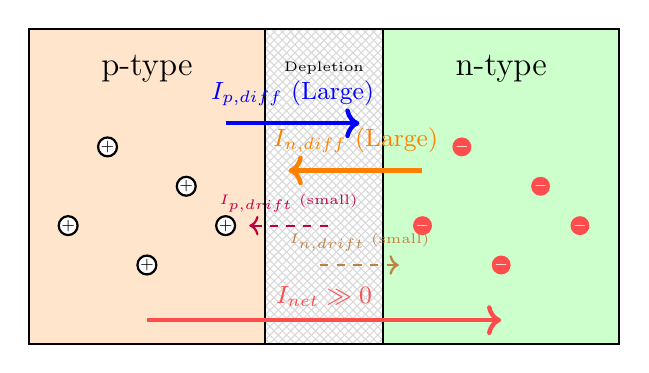
\begin{tikzpicture}[scale=1.0]
        % p-type region
        \draw[thick, fill=orange!20] (0,0) rectangle (3,4);
        \node[font=\large] at (1.5,3.5) {p-type};
        
        % Narrower depletion region
        \draw[thick, fill=yellow!30, pattern=crosshatch, pattern color=gray!30] (3,0) rectangle (4.5,4);
        \node[font=\tiny] at (3.75,3.5) {Depletion};
        
        % n-type region
        \draw[thick, fill=green!20] (4.5,0) rectangle (7.5,4);
        \node[font=\large] at (6,3.5) {n-type};
        
        % Many holes in p-region
        \foreach \x/\y in {0.5/1.5, 1.0/2.5, 1.5/1.0, 2.0/2.0, 2.5/1.5} {
            \draw[fill=white, thick] (\x,\y) circle (0.12cm) node[black, font=\tiny] {$+$};
        }
        
        % Many electrons in n-region
        \foreach \x/\y in {5.0/1.5, 5.5/2.5, 6.0/1.0, 6.5/2.0, 7.0/1.5} {
            \fill[red!70] (\x,\y) circle (0.12cm);
            \node[white, font=\tiny] at (\x,\y) {$-$};
        }
        
        % LARGE diffusion currents (dominate)
        \draw[->, ultra thick, blue] (2.5,2.8) -- (4.2,2.8);
        \node[above, font=\small, blue] at (3.35,2.9) {$I_{p,diff}$ (Large)};
        
        \draw[->, ultra thick, orange] (5.0,2.2) -- (3.3,2.2);
        \node[above, font=\small, orange] at (4.15,2.3) {$I_{n,diff}$ (Large)};
        
        % Small drift currents
        \draw[->, thick, purple, dashed] (3.8,1.5) -- (2.8,1.5);
        \node[above, font=\tiny, purple] at (3.3,1.55) {$I_{p,drift}$ (small)};
        
        \draw[->, thick, brown, dashed] (3.7,1.0) -- (4.7,1.0);
        \node[above, font=\tiny, brown] at (4.2,1.05) {$I_{n,drift}$ (small)};
        
        % Net current
        \draw[->, ultra thick, red!70] (1.5,0.3) -- (6,0.3);
        \node[above, font=\small, red!70] at (3.75,0.35) {$I_{net} \gg 0$};
        
    \end{tikzpicture}
    \end{center}
    
    \vspace{-0.2cm}
    
    \begin{block}{Forward Bias Current}
        \begin{itemize}
            \item \textbf{Diffusion dominates}: $I_{diff} \gg I_{drift}$
            \item \textbf{Holes injected} from p $\rightarrow$ n (minority carriers in n-side)
            \item \textbf{Electrons injected} from n $\rightarrow$ p (minority carriers in p-side)
            \item \textbf{Large current}: $I = I_S(e^{V_A/V_T} - 1) \approx I_S e^{V_A/V_T}$ for $V_A > 0$
        \end{itemize}
    \end{block}
    
\end{frame}

\section{Reverse Bias}

\begin{frame}{Reverse Bias: Circuit Configuration}
    
    \begin{columns}[t]
    \column{0.48\textwidth}
        \textbf{Definition}:
        \begin{itemize}
            \item Connect negative terminal to p-side
            \item Connect positive terminal to n-side
            \item Applied voltage: $V_A < 0$
        \end{itemize}
        
        \vspace{0.3cm}
        
        \textbf{Effect on Junction}:
        \begin{itemize}
            \item Increases barrier height
            \item Barrier becomes: $q(V_{bi} - V_A) = q(V_{bi} + |V_A|)$
            \item Prevents carrier injection
            \item Very small current (leakage)
        \end{itemize}
        
    \column{0.48\textwidth}
        \begin{center}
        \begin{circuitikz}[scale=0.8]
            % Battery (reversed)
            \draw (0,0) to[battery1, l=$V_A < 0$, invert] (0,2);
            
            % PN junction diode
            \draw (0,2) -- (1,2);
            \draw (1,0.5) rectangle (2,3.5);
            \fill[orange!20] (1,0.5) rectangle (1.5,3.5);
            \fill[green!20] (1.5,0.5) rectangle (2,3.5);
            \node at (1.25,2) {p};
            \node at (1.75,2) {n};
            \draw (2,2) -- (3,2);
            
            % Complete circuit
            \draw (3,2) -- (3,0) -- (0,0);
            
            % Labels (reversed)
            \node[above] at (0.5,2.1) {$-$};
            \node[above] at (2.5,2.1) {$+$};
            
            % Very small current
            \draw[->, thick, red, dashed] (1,3.8) -- (2,3.8);
            \node[right, font=\small] at (1,4.2) {$I \approx 0$};
            
        \end{circuitikz}
        \end{center}
        
        % \vspace{0.3cm}
        
        \begin{block}{Key Point}
            Reverse bias \textbf{increases} the potential barrier, preventing majority carrier flow. Only small leakage current flows.
        \end{block}
        
    \end{columns}
    
\end{frame}

\begin{frame}{Reverse Bias: Energy Band Diagram}
    
    \begin{center}
    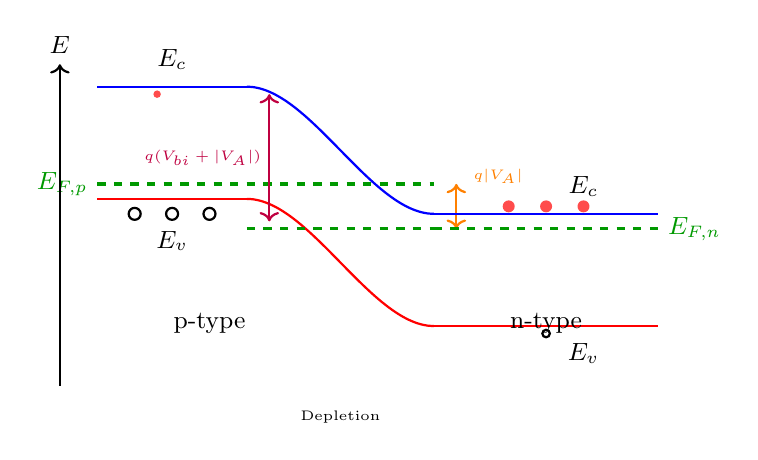
\begin{tikzpicture}[scale=0.95]
        % p-type region
        \begin{scope}[xshift=0cm]
            \draw[thick, blue] (0,3) -- (2,3);
            \node[above, font=\small] at (1,3.1) {$E_c$};
            
            \draw[thick, red] (0,1.5) -- (2,1.5);
            \node[below, font=\small] at (1,1.2) {$E_v$};
            
            % Fermi level
            \draw[very thick, green!60!black, dashed] (0,1.7) -- (2,1.7);
            \node[left, font=\small, green!60!black] at (0,1.7) {$E_{F,p}$};
            
            \foreach \x in {0.5,1.0,1.5} {
                \draw[fill=white, thick] (\x,1.3) circle (0.08cm);
            }
            
            \fill[red!70] (0.8,2.9) circle (0.05cm);
            
            \node[below, font=\small] at (1.5,0.1) {p-type};
        \end{scope}
        
        % Depletion region - INCREASED barrier
        \begin{scope}[xshift=0cm]
            % Increased band bending (1.7 eV instead of 1.1 eV)
            \draw[thick, blue, domain=2:4.5, samples=30, smooth] 
                plot (\x, {3 - 1.7*(3*(((\x-2)/2.5)^2) - 2*(((\x-2)/2.5)^3))});
            
            \draw[thick, red, domain=2:4.5, samples=30, smooth] 
                plot (\x, {1.5 - 1.7*(3*(((\x-2)/2.5)^2) - 2*(((\x-2)/2.5)^3))});
            
            % Fermi levels split (p-side higher, n-side lower for reverse bias)
            \draw[very thick, green!60!black, dashed] (2,1.7) -- (4.5,1.7);
            \draw[very thick, green!60!black, dashed] (2,1.1) -- (4.5,1.1);
            
            \node[below, font=\tiny] at (3.25,-1.2) {Depletion};
            
            % Increased barrier
            \draw[<->, thick, purple] (2.3,1.2) -- (2.3,2.9);
            \node[right, font=\tiny, purple] at (0.5,2.05) {$q(V_{bi}+|V_A|)$};
            
            % Applied voltage arrow (between the two Fermi levels)
            \draw[<->, thick, orange] (4.8,1.1) -- (4.8,1.7);
            \node[right, font=\tiny, orange] at (4.9,1.8) {$q|V_A|$};
        \end{scope}
        
        % n-type region
        \begin{scope}[xshift=0cm]
            \draw[thick, blue] (4.5,1.3) -- (7.5,1.3);
            \node[above, font=\small] at (6.5,1.4) {$E_c$};
            
            \draw[thick, red] (4.5,-0.2) -- (7.5,-0.2);
            \node[below, font=\small] at (6.5,-0.3) {$E_v$};
            
            \draw[very thick, green!60!black, dashed] (4.5,1.1) -- (7.5,1.1);
            \node[right, font=\small, green!60!black] at (7.5,1.1) {$E_{F,n}$};
            
            \foreach \x in {5.5,6.0,6.5} {
                \fill[red!70] (\x,1.4) circle (0.08cm);
            }
            
            \draw[fill=white, thick] (6.0,-0.3) circle (0.05cm);
            
            \node[below, font=\small] at (6.0,0.1) {n-type};
        \end{scope}
        
        \draw[->, thick] (-0.5,-1) -- (-0.5,3.3) node[above, font=\small] {$E$};
        
    \end{tikzpicture}
    \end{center}
    
    \begin{itemize}
        \item \textbf{Increased barrier}: From $qV_{bi}$ to $q(V_{bi} + |V_A|)$
        \item \textbf{Split Fermi levels}: $E_{F,n} - E_{F,p} = q|V_A|$ (reversed from forward bias)
        \item \textbf{Wider depletion region}: More space charge
    \end{itemize}
    
\end{frame}

\begin{frame}{Reverse Bias: Current Flow}
    
    \begin{center}
    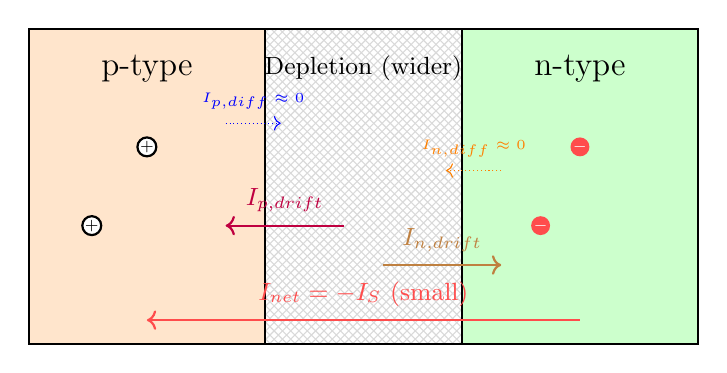
\begin{tikzpicture}[scale=1.0]
        % p-type region
        \draw[thick, fill=orange!20] (0,0) rectangle (3,4);
        \node[font=\large] at (1.5,3.5) {p-type};
        
        % Wider depletion region
        \draw[thick, fill=yellow!30, pattern=crosshatch, pattern color=gray!30] (3,0) rectangle (5.5,4);
        \node[font=\small] at (4.25,3.5) {Depletion (wider)};
        
        % n-type region
        \draw[thick, fill=green!20] (5.5,0) rectangle (8.5,4);
        \node[font=\large] at (7,3.5) {n-type};
        
        % Few holes in p-region
        \foreach \x/\y in {0.8/1.5, 1.5/2.5} {
            \draw[fill=white, thick] (\x,\y) circle (0.12cm) node[black, font=\tiny] {$+$};
        }
        
        % Few electrons in n-region
        \foreach \x/\y in {6.5/1.5, 7.0/2.5} {
            \fill[red!70] (\x,\y) circle (0.12cm);
            \node[white, font=\tiny] at (\x,\y) {$-$};
        }
        
        % Very small diffusion (nearly zero)
        \draw[->, thin, blue, densely dotted] (2.5,2.8) -- (3.2,2.8);
        \node[above, font=\tiny, blue] at (2.85,2.85) {$I_{p,diff} \approx 0$};
        
        \draw[->, thin, orange, densely dotted] (6.0,2.2) -- (5.3,2.2);
        \node[above, font=\tiny, orange] at (5.65,2.25) {$I_{n,diff} \approx 0$};
        
        % Small drift current (reverse saturation)
        \draw[->, thick, purple] (4.0,1.5) -- (2.5,1.5);
        \node[above, font=\small, purple] at (3.25,1.55) {$I_{p,drift}$};
        
        \draw[->, thick, brown] (4.5,1.0) -- (6.0,1.0);
        \node[above, font=\small, brown] at (5.25,1.05) {$I_{n,drift}$};
        
        % Net current (small, reverse direction)
        \draw[<-, thick, red!70] (1.5,0.3) -- (7.0,0.3);
        \node[above, font=\small, red!70] at (4.25,0.35) {$I_{net} = -I_S$ (small)};
        
    \end{tikzpicture}
    \end{center}
    
    \vspace{-0.2cm}
    
    \begin{block}{Reverse Bias Current}
        \begin{itemize}
            \item \textbf{Diffusion blocked}: Potential Energy barrier too high for majority carriers to diffuse
            \item \textbf{Drift dominates}: Minority carriers swept across junction by E field
            \item \textbf{Reverse saturation current}: $I \approx -I_S$ (constant, small)
            \item Typically: $I_S \sim 10^{-12}$ to $10^{-15}$ A (pA to fA range)
        \end{itemize}
    \end{block}
    
\end{frame}

\section{Diode I-V Characteristic}

\begin{frame}{The Shockley Diode Equation}
    
    \begin{columns}[t]
    \column{0.48\textwidth}
        \begin{block}{Diode Equation}
            $$I = I_S \left(e^{V_A/V_T} - 1\right)$$
            where:
            \begin{itemize}
                \item $I_S$ = reverse saturation current
                \item $V_A$ = applied voltage
                \item $V_T = \frac{kT}{q} \approx 26$ mV at 300K
            \end{itemize}
        \end{block}
        
        \vspace{0.3cm}
        
        \textbf{Forward Bias} ($V_A > 0$):
        $$I \approx I_S e^{V_A/V_T}$$
        \begin{itemize}
            \item Exponential increase
            \item Large current for small voltage
        \end{itemize}
        
        \vspace{0.3cm}
        
        \textbf{Reverse Bias} ($V_A < 0$, $|V_A| \gg V_T$):
        $$I \approx -I_S$$
        \begin{itemize}
            \item Constant small current
            \item Independent of voltage
        \end{itemize}
        
    \column{0.48\textwidth}
        \begin{center}
        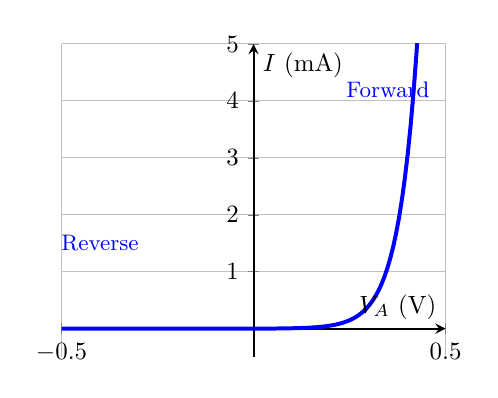
\begin{tikzpicture}[scale=0.9]
        \begin{axis}[
            width=7cm, height=6cm,
            xlabel={$V_A$ (V)},
            ylabel={$I$ (mA)},
            xlabel style={at={(axis description cs:1,0)}, anchor=west},
            ylabel style={at={(axis description cs:0,1)}, anchor=south},
            xmin=-0.5, xmax=0.5,
            ymin=-0.5, ymax=5,
            xtick={-0.5, 0, 0.5},
            ytick={0, 1, 2, 3, 4, 5},
            grid=major,
            axis lines=middle,
            thick,
            restrict y to domain=-1:10,
        ]
        
        % Forward bias (exponential)
        \addplot[blue, ultra thick, domain=0:0.75, samples=100] 
            {0.001*exp(x/0.05) - 0.001};
        
        % Reverse bias (flat at -I_S)
        \addplot[blue, ultra thick, domain=-1:0, samples=50] 
            {0.001*exp(x/0.05) - 0.001};
        
        % Label regions
        \node[font=\small, blue] at (axis cs:0.35,4.2) {Forward};
        \node[font=\small, blue] at (axis cs:-0.4,1.5) {Reverse};
        
        \end{axis}
        \end{tikzpicture}
        \end{center}
        
    \end{columns}
    
\end{frame}

\section{Breakdown}

\begin{frame}{Reverse Bias Breakdown}
    
    \begin{columns}[t]
    \column{0.48\textwidth}
        \textbf{What is Breakdown?}
        \begin{itemize}
            \item Large reverse voltage applied
            \item Barrier becomes very large
            \item Depletion region very wide
            \item Electric field becomes extremely high
            \item Sudden large reverse current
        \end{itemize}
        
        \vspace{0.3cm}
        
        \textbf{Breakdown Voltage} $V_{BR}$:
        \begin{itemize}
            \item Voltage at which breakdown occurs
            \item Depends on doping concentration
            \item Higher doping $\rightarrow$ lower $V_{BR}$
            \item Typical: 50V to 1000V
            \item Zener diodes: 2V to 200V
        \end{itemize}
        
    \column{0.48\textwidth}
        \begin{center}
        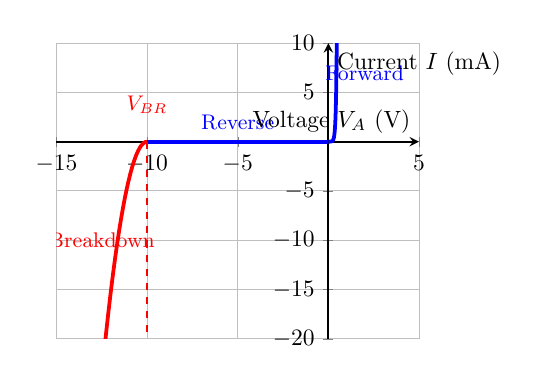
\begin{tikzpicture}[scale=0.85]
        \begin{axis}[
            width=7cm, height=6cm,
            xlabel={Voltage $V_A$ (V)},
            ylabel={Current $I$ (mA)},
            xmin=-15, xmax=5,
            ymin=-20, ymax=10,
            xtick={-15, -10, -5, 0, 5},
            ytick={-20, -15, -10, -5, 0, 5, 10},
            grid=major,
            axis lines=middle,
            thick,
            restrict y to domain=-25:15,
        ]
        
        % Forward bias
        \addplot[blue, ultra thick, domain=0:0.75, samples=50] 
            {0.001*exp(x/0.05) - 0.001};
        
        % Reverse bias (flat)
        \addplot[blue, ultra thick, domain=-10:0, samples=50] 
            {-0.001};
        
        % Breakdown region (extended to reach -19 mA)
        \addplot[red, ultra thick, domain=-15:-10, samples=50] 
            {-0.001 - 3.8*(x+10)^2};
        
        % Breakdown voltage line
        \draw[dashed, red] (axis cs:-10,0) -- (axis cs:-10,-20);
        \node[above, font=\small, red] at (axis cs:-10,2) {$V_{BR}$};
        
        % Labels
        \node[font=\small, blue] at (axis cs:2,7) {Forward};
        \node[font=\small, blue] at (axis cs:-5,2) {Reverse};
        \node[font=\small, red] at (axis cs:-12.5,-10) {Breakdown};
        
        \end{axis}
        \end{tikzpicture}
        \end{center}
        
    \end{columns}
    
\end{frame}

\begin{frame}{Breakdown Mechanisms}
    
    \begin{columns}[t]
    \column{0.48\textwidth}
        \textbf{1. Zener Breakdown}
        
        \begin{itemize}
            \item Quantum tunneling effect
            \item Electrons tunnel through barrier
            \item Direct band-to-band tunneling
        \end{itemize}
        
        \vspace{-0.2cm}
        
        \begin{center}
        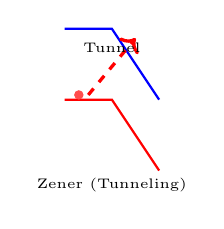
\begin{tikzpicture}[scale=0.6]
            % Simplified band diagram showing tunneling
            \draw[thick, blue] (0,2) -- (1,2) -- (2,0.5);
            \draw[thick, red] (0,0.5) -- (1,0.5) -- (2,-1);
            
            % Electron in VB
            \fill[red!70] (0.3,0.6) circle (0.1cm);
            
            % Tunneling arrow
            \draw[->, very thick, red, dashed] (0.5,0.6) -- (1.5,1.8);
            \node[above, font=\tiny] at (1,1.3) {Tunnel};
            
            % Labels
            \node[font=\tiny] at (1,-1.3) {Zener (Tunneling)};
        \end{tikzpicture}
        \end{center}
        
    \column{0.48\textwidth}
        \textbf{2. Avalanche Breakdown}
        
        \begin{itemize}
            \item Higher breakdown voltage ($V_{BR} > 5$V)
            \item Accelerated carriers create e-h pairs
            \item Chain reaction (avalanche)
        \end{itemize}
        
        \vspace{-0.2cm}
        
        \begin{center}
        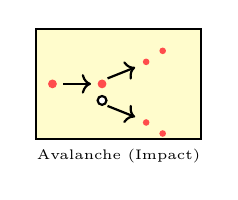
\begin{tikzpicture}[scale=0.7]
            % Depletion region
            \draw[thick, fill=yellow!20] (0,0) rectangle (3,2);
            
            % Initial electron
            \fill[red!70] (0.3,1) circle (0.08cm);
            \draw[->, thick] (0.5,1) -- (1.0,1);
            
            % First impact
            \fill[red!70] (1.2,1) circle (0.08cm);
            \draw[fill=white, thick] (1.2,0.7) circle (0.08cm);
            \draw[->, thick] (1.3,1.1) -- (1.8,1.3);
            \draw[->, thick] (1.3,0.6) -- (1.8,0.4);
            
            % More impacts
            \foreach \x/\y in {2.0/1.4, 2.0/0.3, 2.3/1.6, 2.3/0.1} {
                \fill[red!70] (\x,\y) circle (0.06cm);
            }
            
            \node[font=\tiny] at (1.5,-0.3) {Avalanche (Impact)};
        \end{tikzpicture}
        \end{center}
        
    \end{columns}
    
    \vspace{-0.3cm}
    
    \begin{block}{Key Differences}
        \begin{itemize}
            \item Zener: Heavy doping, low $V_{BR}$, tunneling
            \item Avalanche: Light doping, high $V_{BR}$, impact ionization
            \item Both produce large reverse current at breakdown
        \end{itemize}
    \end{block}
    
\end{frame}

\section{Summary}

\begin{frame}{Summary: PN Junction Under Bias}
    
    \begin{columns}[t]
    \column{0.48\textwidth}
        \begin{enumerate}
            \item \textbf{Equilibrium (No Bias)}:
            \begin{itemize}
                \item Flat Fermi level, $V_A = 0$
                \item Barrier: $qV_{bi}$
                \item No net current
            \end{itemize}
            
            \vspace{0.3cm}
            
            \item \textbf{Forward Bias} ($V_A > 0$):
            \begin{itemize}
                \item Reduced barrier: $q(V_{bi} - V_A)$
                \item Large diffusion current
                \item $I \approx I_S e^{V_A/V_T}$
                \item Narrower depletion region
            \end{itemize}
        \end{enumerate}
        
    \column{0.48\textwidth}
        \begin{enumerate}
            \setcounter{enumi}{2}
            \item \textbf{Reverse Bias} ($V_A < 0$):
            \begin{itemize}
                \item Increased barrier: $q(V_{bi} + |V_A|)$
                \item Small drift current
                \item $I \approx -I_S$ (constant)
                \item Wider depletion region
            \end{itemize}
            
            \vspace{0.3cm}
            
            \item \textbf{Breakdown} ($V_A < -V_{BR}$):
            \begin{itemize}
                \item Zener: Tunneling (heavy doping, low $V_{BR}$)
                \item Avalanche: Impact ionization (light doping, high $V_{BR}$)
                \item Used in Zener diodes for voltage regulation
            \end{itemize}
        \end{enumerate}
        
    \end{columns}
    
\end{frame}

\begin{frame}{Key Formulas and Parameters}
    
    \begin{columns}[T]
    \column{0.48\textwidth}
    \begin{table}[t]
    \centering
    \renewcommand{\arraystretch}{1.8}
    \small
    \begin{tabular}{|l|c|}
    \hline
    \textbf{Parameter} & \textbf{Formula} \\
    \hline
    \hline
    Diode current & $I = I_S(e^{V_A/V_T} - 1)$ \\
    \hline
    Thermal voltage & $V_T = \dfrac{kT}{q} \approx 26$ mV \\
    \hline
    Forward bias & $I \approx I_S e^{V_A/V_T}$ \\
    \hline
    Reverse bias & $I \approx -I_S$ \\
    \hline
    \end{tabular}
    \end{table}
    
    \column{0.48\textwidth}
    \begin{table}[t]
    \centering
    \renewcommand{\arraystretch}{1.8}
    \small
    \begin{tabular}{|l|c|}
    \hline
    \textbf{Parameter} & \textbf{Value/Condition} \\
    \hline
    \hline
    Turn-on voltage & $V_{on} \approx 0.7$ V (Si) \\
    \hline
    Sat. current & $I_S \sim 10^{-12}$ A \\
    \hline
    Breakdown & $V_A < -V_{BR}$ \\
    \hline
    Zener range & 2V -- 200V \\
    \hline
    \end{tabular}
    \end{table}
    \end{columns}
    
    \vspace{-0.3cm}
    
    \begin{block}{Important Concepts}
        \begin{itemize}
            \item Forward bias: Exponential $I$-$V$ relationship
            \item Reverse bias: Nearly constant current $-I_S$
            \item Breakdown: Controlled in Zener diodes, destructive in regular diodes
            \item Depletion width: Varies with applied voltage
        \end{itemize}
    \end{block}
    
\end{frame}

\end{document}
